Usualmente, motores alimentados por retificadores ou conversores CC-CC podem ter sua velocidade e corrente controladas. Com isso, é possível obter maior precisão no controle de velocidade, melhor resposta dinâmica, menor sensibilidade a variações de torque da carga, controle da corrente máxima nos semicondutores de potência e no motor e também a limitação no torque máximo produzido pelo motor e na aceleração máxima na carga.

\subsubsection{Modelo do motor e do conversor}

A figura \ref{fig:C1_42} apresenta o circuito equivalente do motor CC.

\begin{figure}[ht!]
\center
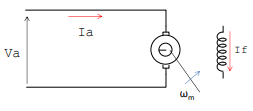
\includegraphics[scale= 1]{imagens/circuito1_42.png}
\caption{\label{fig:C1_42}Circuito equivalente motor CC.}
\caption*{Fonte: MARTINS, cap. 2, eslaide 13.}
\end{figure}

Para esse circuito, se aplica a função de transferência conforme no diagrama da figura \ref{fig:DBMCC}.

\begin{figure}[ht!]
\center
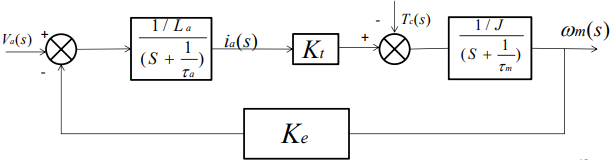
\includegraphics[scale= 0.88]{imagens/diagrama1_42.png}
\caption{\label{fig:DBMCC}Diagrama de blocos do motor CC.}
\caption*{Fonte: MARTINS, cap. 2, eslaide 13.}
\end{figure}

Levando $T_{C}(s)$ a zero na figura \ref{fig:D1_42}, obtém-se 
\[\frac{\omega_{m}(s)}{V_{a}(s)} =  \frac{k_{t}}{L_{a}J\left[\left(s + \frac{1}{\tau_{a}}\right)\left(s + \frac{1}{\tau_{m}}\right) + \frac{1}{\tau_{a}\tau_{ml}}\right] }.\]
I.e., a figura \ref{fig:D2_42} representa o funcionamento do motor.

\begin{figure}[ht!]
\center
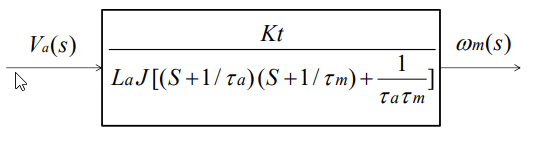
\includegraphics[scale= 0.88]{imagens/diagrama2_42.png}
\caption{\label{fig:D2_42}Diagrama de blocos compactado do motor CC.}
\caption*{Fonte: MARTINS, cap. 2, eslaide 14.}
\end{figure}

Sabendo que a condução do conversor é contínua e ignorando o atraso induzido pelo mesmo, tem-se a representação em diagrama de blocos conforme na figura \ref{fig:D3_42}, cuja função de transferência é 
\[\frac{V_{a}(s)}{E_{c}(s)} = k_{c}.\]
Portanto, a função de transferência do conjunto conversor-motor será como ilustrado na figura \ref{fig:D1_42}.

\begin{figure}[ht!]
\center
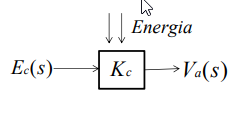
\includegraphics[scale= 0.88]{imagens/diagrama3_42.png}
\caption{\label{fig:D3_42}Representação idealizada do conversor estático que alimenta o motor CC.}
\caption*{Fonte: MARTINS, cap. 2, eslaide 15.}
\end{figure}

\begin{figure}[ht!]
\center
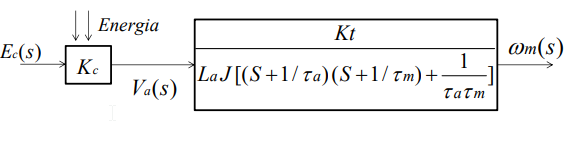
\includegraphics[scale= 0.88]{imagens/diagrama4_42.png}
\caption{\label{fig:D1_42} Diagrama de blocos do conversor alimentando o motor CC.}
\caption*{Fonte: MARTINS, cap. 2, eslaide 15.}
\end{figure}

\subsubsection{Regulação de velocidade}

Quando se realiza um sensor de velocidade e um regulador de velocidade, o controle de velocidade em malha fechada é viável. Nesse caso, o diagrama de blocos é conforme ilustrado na figura \ref{fig:D1_43}.

\begin{figure}[ht!]
\center
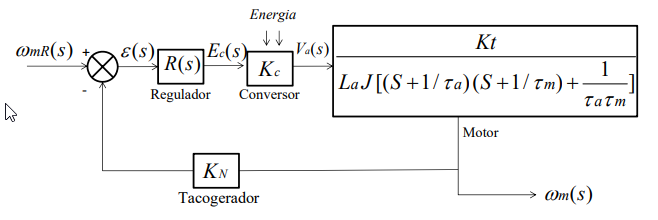
\includegraphics[scale= 0.88]{imagens/diagrama1_43.png}
\caption{\label{fig:D1_43} Diagrama de blocos do conjunto motor CC e conversor estático com regulador de velocidade.}
\caption*{Fonte: MARTINS, cap. 2, eslaide 16.}
\end{figure} 
 
Um regulador proporcional, regido por
 \[R(s) = k_{R}\]
não altera a ordem do sistema e possui um erro de posição inversamente proporcional ao ganho do regulador.
 
Já um regulador proporcional-integral, de forma
\[R(s) = k_{R}\frac{\left(1+s+\tau_{R}\right)}{s\tau_{R}}\]
possui erro de posição nulo e maior precisão estática no controle, sendo que $k_{R}$ pode assumir valores menores do que no caso puramente proporcional.

\subsubsection{Regulação de corrente}

Com um erro de velocidade grande, o sistema de controle resulta em valores altos de corrente de armadura. A função de transferência é representada na figura \ref{fig:D1_44}. Pode-se representar um regulador de corrente como na figura \ref{fig:D2_44}.

\begin{figure}[ht!]
\center
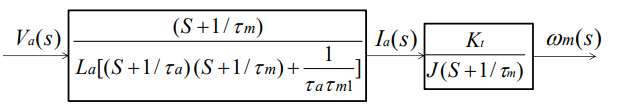
\includegraphics[scale= 0.88]{imagens/diagrama1_44.png}
\caption{\label{fig:D1_44}Outra forma de representar o motor CC em diagrama de blocos.}
\end{figure} 

\begin{figure}[ht!]
\center
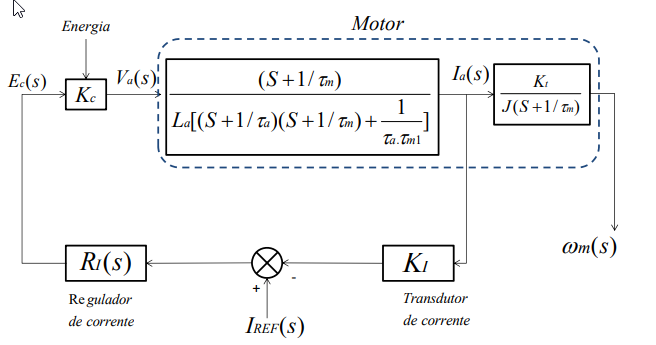
\includegraphics[scale= 0.88]{imagens/diagrama2_44.png}
\caption{\label{fig:D2_44}Diagrama de blocos do  motor CC e conversor estático com regulador de corrente.}
\caption*{Fonte: MARTINS, cap. 2, eslaide 19.}
\end{figure} 

Aqui, $R_{l}(s)$ representa o regulador de corrente. Também é possível implementar para tal um regulador proporcional ou um proporcional-integral. A limitação de $I_{a}(s)$ é dada pelo limite do valor máximo da corrente de referência $I_{REF}(s)$.

Caso ambos os reguladores de velocidade e de corrente sejam utilizados, basta limitar o erro de velocidade para limitar $I_{a}(s)$, como ilustra a figura \ref{fig:D3_44}. Esse método é conhecido como regulação em cascata.

\begin{figure}[ht!]
\center
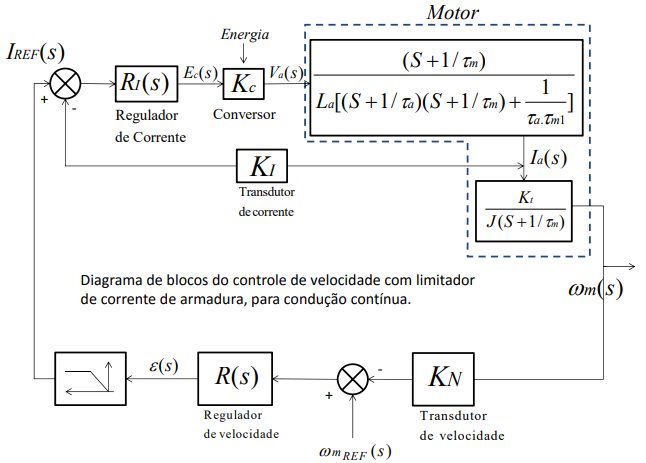
\includegraphics[scale= 0.88]{imagens/diagrama3_44.png}
\caption{\label{fig:D3_44}Diagrama de blocos do controle de velocidade com limitador de corrente de armadura, para condução contínua.}
\caption*{Fonte: MARTINS, cap. 2, eslaide 21.}
\end{figure} 

\subsubsection{Monitoração da velocidade}

Uma forma de monitorar a velocidade é através da força eletromotriz produzida pelo motor, como ilustra a figura \ref{fig:C1_45}). Considerando uma excitação constante,
\[E_{a} = k_{a}\omega_{m} = V_{m} - R_{a}I_{a}.\]

\begin{figure}[ht!]
\center
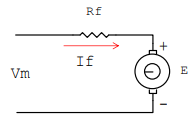
\includegraphics[scale= 0.88]{imagens/circuito_45.png}
\caption{\label{fig:C1_45} Método da força eletromotriz.}
\caption*{Fonte: MARTINS, cap. 2, eslaide 22.}
\end{figure} 

Na figura \ref{fig:C2_45} pode-se obter o valor de $E_{a}$ e da corrente (resistor em série com a a armadura). Logo, a tensão proporcional do motor é obtida simplesmente na saída do amplificador.

\begin{figure}[ht!]
\center
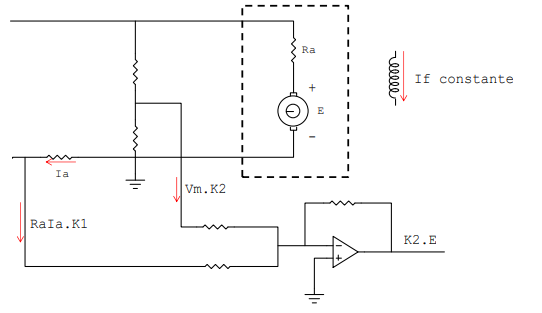
\includegraphics[scale= 0.88]{imagens/circuito2_45.png}
\caption{\label{fig:C2_45} Medida indireta da força eletro-motriz.}
\caption*{Fonte: MARTINS, cap. 2, eslaide 23.}
\end{figure} 

Uma outra forma de monitorar a velocidade é usando um tacogerador, que fornece maior precisão no controle de velocidade pois possui excelente linearidade. Esse método produz ruídos com frequência e amplitude proporcionais à velocidade. No caso de velocidades baixas, onde o uso de filtros interfere na resposta do sistema, emprega-se tacogeradores de grande diâmetro com muitas lâminas no comutador. Tacogeradores digitas são ainda mais precisos do que os de tensão contínua.

\subsubsection{Sensores de corrente}

Uma abordagem para o monitoramento de corrente é utilizando transdutores de corrente alternada, utilizando-se um transformador de corrente no lugar de corrente alternada do conversor, como ilustra a figura \ref{fig:C1_46}. Veja que esse método não é aplicável na presença de um diodo de roda livre.

\begin{figure}[ht!]
\center
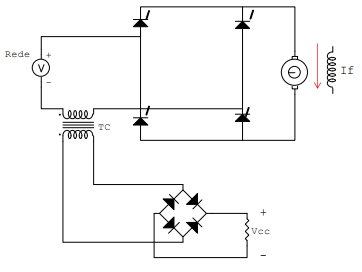
\includegraphics[scale= 0.88]{imagens/circuito1_46.png}
\caption{\label{fig:C1_46}Uso de transformador de corrente no lado CA do conversor.}
\caption*{Fonte: MARTINS, cap. 2, eslaide 25.}
\end{figure} 

A abordagem mais econômica é através de um sensor resistivo, apesar da tensão de nível ser muito baixa. Além disso, o sinal não é eletricamente isolado da parte de potência, o que é uma desvantagem.

Já o transdutor magnético de corrente contínua produz um resistência $R$ proporcional à corrente $I_{a}$. Seu princípio é ilustrado na figura \ref{fig:C2_46}.

\begin{figure}[ht!]
\center
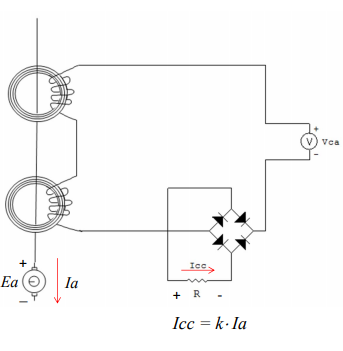
\includegraphics[scale= 0.88]{imagens/circuito2_46.png}
\caption{\label{fig:C2_46} Transdutor magnético de corrente contínua.}
\caption*{Fonte: MARTINS, cap. 2, eslaide 27.}
\end{figure} 

São aplicados núcleos toroidais de Permalloy, uma liga de ferro-níquel que possui poucas perdas magnéticas e uma permeabilidade alta.

Por fim, é possível também utilizar um transdutor eletrônico CC. O diagrama de blocos da figura \ref{fig:D1_46} demonstra o princípio de funcionamento dessa abordagem.

\begin{figure}[ht!]
\center
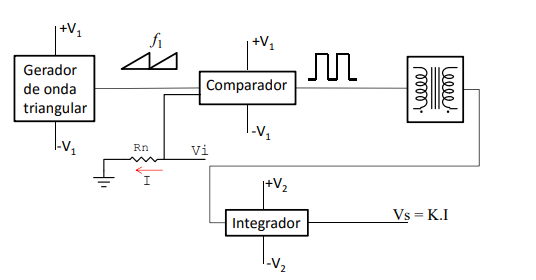
\includegraphics[scale= 0.88]{imagens/diagrama1_46.png}
\caption{\label{fig:D1_46} Transdutor eletrônico de corrente contínua.}
\caption*{Fonte: MARTINS, cap. 2, eslaide 28.}
\end{figure}

$V(s)$ é proporcional ao valor médio da corrente $I$. As fontes $V_{1}$ e $V_{2}$ são isolados entre si. Dessa forma $V_{s}$ também é isolado de $V_{i}$. Por possuir uma frequência $f_{t}$ elevada, esse transdutor possui uma resposta muito rápida. Além disso, é eletronicamente simples e compacto. Vários conversores comerciais possuem esse transdutor.

Um outro tipo de sensor disponível são os sensores a efeito Hall, que apresentam excelente precisão, mas alto custo e difícil implementação (figura \ref{fig:F1_46}).
\[V_{H} = KBI.\]

\begin{figure}[ht!]
\center
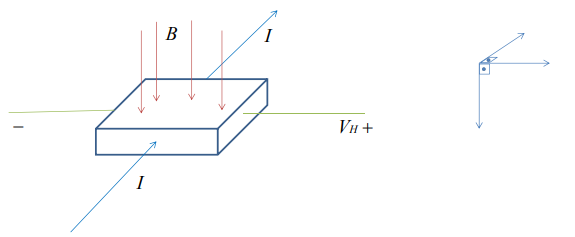
\includegraphics[scale= 0.88]{imagens/figura1_46.png}
\caption{\label{fig:F1_46} Semicondutor submetido a uma indução magnética B e percorrido por uma corrente i}
\caption*{Fonte: MARTINS, cap. 2, eslaide 30.}
\end{figure}

\subsubsection{Reguladores em paralelo}

Em um sistema de regulação em cascata, geralmente é difícil atingir um comportamento dinâmico ótimo, uma vez que dois reguladores influenciam ao mesmo tempo. Assim, costumeiramente utilizam-se os reguladores em paralelo, como ilustra a figura \ref{fig:D1_47}.

\begin{figure}[ht!]
\center
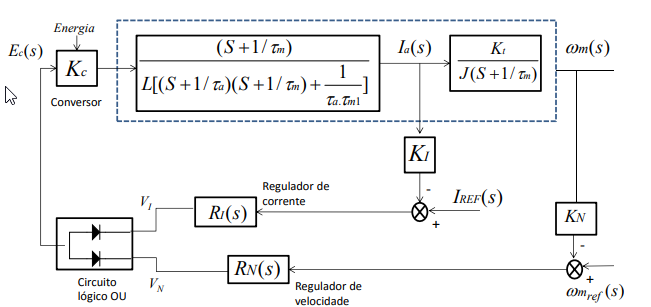
\includegraphics[scale= 0.88]{imagens/diagrama1_47.png}
\caption{\label{fig:D1_47} Motor de corrente contínua controlado por regulador em paralelo.}
\caption*{Fonte: MARTINS, cap. 2, eslaide 32.}
\end{figure}

